\documentclass[12pt,letter]{article}

%compile with pdflatex:
%:! bibtex %:r
%:! pdflatex -synctex=1 -interaction=nonstopmode --shell-escape %

\usepackage{amsmath}
\usepackage{natbib}
\usepackage{graphicx}
\usepackage{hyperref}
\usepackage{subcaption}
\usepackage{caption}
\captionsetup{font={sf,small},labelfont=bf,width=0.95\textwidth}

\usepackage{titlesec}
\titleformat*{\section}{\large\bfseries} %LARGE, Large, large
\titleformat*{\subsection}{\normalsize\bfseries} %LARGE, Large, large
\usepackage{booktabs}
\newcommand{\tabitem}{~~\llap{\textbullet}~~}

\title{Uses of kernel statistics on volcanic vents}
\date{}
\author{}

\usepackage[margin=1in]{geometry}
\usepackage{setspace}
%\doublespacing

\usepackage{lineno}
%\linenumbers

\usepackage{titlesec}
\titleformat*{\section}{\large\bfseries} %LARGE, Large, large
\titleformat*{\subsection}{\normalsize\bfseries} %LARGE, Large, large

\begin{document}

\maketitle

\section{Introduction}

What is important about:
\begin{enumerate}
\item The size of volcano clusters?
\item The density of vents within clusters?
\item The volume density within clusters?
\end{enumerate}

Who has tackled these questions before, who has tried to figure out spatial statistics
of volcanic fields? What is the strength and weakness of different methods?


\subsection{Kernel Density Estimation}
Commonly in geology, physical processes create a partially random population of point features, such as sinkholes, volcanoes, or kettle lakes. The spatial distribution of these point features is governed by an underlying physical process, and the physical process can often be modeled to create a probability model of where points are more likely to be created. For instance, sinkholes are more likely to occur in locations where soluble carbonate rock is at or near the water table, so a map showing the probability of sinkhole development might reflect the distribution of shallow carbonate rocks. In contrast, volcanoes are formed from a magma source. If the location, depth, and productivity of the magma source is well known, models can be made to map the potential locations of volcanism on the Earth's surface, where a higher likelihood of eruption would be over the most productive locations of the magma source region. 

Unfortunately for volcanologists, the distribution and characteristics of magma sources in the ground are generally far less well constrained than the distribution of volcanoes on the Earth's surface. Instead of creating a probabilistic spatial model of volcanic events using knowledge of the magma source, the existing distribution of volcanoes can be used. Using only the point locations of volcanoes, one might conclude that new volcanoes are likely to form in areas where more volcanoes already exist, where the spatial density of volcanoes is higher. This is an attempt to estimate the physical model of volcano production when knowledge of the underlying physical process is limited.

The process of estimating the ``true'' point density distribution by assigning probability density functions (PDFs) to a population of randomly sampled points from this distribution is called Kernel Density Estimation (KDE). A kernel is an identical PDF assigned to points to describe their influence on their surrounding region. Essentially, If the kernel is the normal distribution centered on a point, the point has more influence at the point's location (at the maximum value of the normal distribution) and influence decreases away from the point following the value of the normal distribution. In KDE, influence becomes density, so that point density is highest at a point location and decreases away from the point, in effect smoothing the point.

Given a map catalog of volcanoes, a density value, $\lambda$, for each volcano can be calculated for any location on the map, using the associated kernel PDF. If the kernel is normally distributed (i.e. Gaussian), the kernel density of a volcano for location with cartesian coordinates ($x$,$y$) is calculated as
\begin{equation}
\lambda(x,y) = \frac{1}{\sigma\sqrt{2\pi}}\exp\left[\frac{-(x-x_v)^2-(y-y_v)^2}{2\sigma^2}\right]
\end{equation}
where ($x_v$,$y_v$) is the coordinate pair of the volcano and $\sigma$ is the PDF standard deviation, or kernel bandwidth. The larger the kernel bandwidth, the further the density of the point is spread across the map. The total volcano point density at this location can be found by summing the point densities of all volcanoes, $i$, in the catalog of $N$ volcanoes:
\begin{equation}
\lambda(x,y) = \frac{1}{N\sigma\sqrt{2\pi}}\sum\limits_{i=1}^{N}\exp\left[\frac{-(x-x_i)^2-(y-y_i)^2}{2\sigma^2}\right].
\label{eq_simpleKDE}
\end{equation}

Kernel PDFs do not have to be axi-symmetric normal distributions. In this paper, a bivariate normal distribution will be used to model density, so kernels will be Gaussian ellipses instead of circles (circular distributions can be considered univariate as they are defined by one standard deviation or bandwidth). These ellipses will also be unconstrained in direction, so their major axes do not have to be aligned in a cardinal direction. This is done by multiplying the distance between locations and volcanoes, treated here a 1x2 distance matrix, by a covariance matrix that defines the standard deviation in the x and y directions and the covariance between these dimensions. The covariance matrix is given as
\begin{equation}\begin{bmatrix}
\sigma_x^2 & \sigma_x\sigma_y\rho\\
\sigma_x\sigma_y\rho & \sigma_y^2
\label{eq_covariance}
\end{bmatrix}\end{equation}
where $\sigma_x$ is the x-direction standard deviation, $\sigma_y$ is the y-direction standard deviation, and $\rho$ is the covariance of these two. A covariance of 0 results in a kernel ellipse with axes aligned with the cardinal directions, while higher covariance skews or rotates the ellipse away from the cardinal directions.

Kernel bandwidth, the amount that the kernel ellipse is smoothed in any given direction, is an important parameter in estimating the unknown density of point features. Again, the point of KDE is to estimate the underlying spatial probability of a point feature (e.g. a volcano) being created, using only the points that can already be observed. Selecting a bandwidth that is too small will overly concentrate volcano density around each existing volcanoes, underestimating the likelihood of a new volcano in between existing edifices. A bandwidth that is too large will overly smooth volcano density, overestimating the likelihood of new volcanic events far from the existing volcano population.

Several bandwidth selectors have been created for KDE and in this project the Summed Asymptotic Means Square Error (SAMSE) selector will be used Duong, 2003). This selector is chosen because it has been validated using point populations of known distributions (Duong, 2007) and it has been shown to be more stable than similar selectors (Duong and Hazelton, 2003). The SAMSE bandwidth selector also is preferred because it provides an unconstrained bandwidth model using the covariance matrix formula in Equation \ref{eq_covariance}.

Calculating the estimated spatial density, $\hat{\lambda}$, of point features in a location, $s$, using the unconstrained, bivariate bandwidth is done by modifying Equation \ref{eq_simpleKDE}, so that
\begin{equation}
\hat{\lambda}(\mathbf{s})=\frac{1}{2N\pi\sqrt{|\mathbf{H}|}}\sum\limits_{i=1}^{N}\exp\left[-\frac{1}{2}\mathbf{b^Tb}\right]
\label{eq_kde}
\end{equation}
where $\mathbf{H}$ is the 2x2 covariance matrix and $|\mathbf{H}|$ is its determinant, $\mathbf{b}=\mathbf{H}^{-0.5}\mathbf{d}$ and $\mathbf{b^T}$ is its transform. $\mathbf{d}$ is the 1x2 distance matrix, with the form
\begin{equation}\begin{bmatrix}
x_s-x_i\\
y_s-y_i
\label{eq_distancematrix}
\end{bmatrix}\end{equation}
where ($x_s$,$y_s$) are the cartesian coordinates of the location of interest and ($x_i$,$y_i$) are the coordinates of the $i^{\text{th}}$ volcano.



\section{Methods}

\subsection{Data collection}
Catalogs of 20 volcano clusters have been collected for this study, including 10 volcanic fields on Earth, 3 on Mars, and 7 on Venus. The volcanoes in all clusters are primarily described as monogenetic, though some clusters are formed nearby or on top of central-vent volcanoes (e.g. Mount Adams, WA and Arsia Mons, Mars).
10 Earth
3 Mars
7 Venus



\begin{table}
\centering
\caption{Distributed-style Volcano Clusters}
\begin{tabular}{p{2cm} p{2.5cm} p{2cm} c c p{4cm}}
\toprule
Cluster	&	Region, &	Location	&	Vent &	Bandwidth	&	Data\\
Name		& Country	&	Lat, Long	&	Count	&	Matrix (km$^2$)	&Source\\
\midrule
Abu$^*$		&	Ch\={u}goku, Japan	&	34$^{\circ}$30'N, 131$^{\circ}$35'E	&	56	&	$\bigl[\begin{smallmatrix} 3.81&0.230\\0.230&2.05 \end{smallmatrix}\bigr]$	&	\citet{kiyosugi2012relationship,kiyosugi2010relationships}\\
Adams		&	Washington, USA	&	46$^{\circ}$10'N, 121$^{\circ}$30'W	&	89	&	$\bigl[\begin{smallmatrix} 3.25&0.989\\0.989&13.9 \end{smallmatrix}\bigr]$	&	\citet{barron2014database}\\
Blk. Rock Desert$^*$ &	Utah, USA		&	39$^{\circ}$N, 112$^{\circ}$30'W&	39	&	$\bigl[\begin{smallmatrix} 3.51&0.500\\0.500&10.6 \end{smallmatrix}\bigr]$	&	\citet{kiyosugi2012relationship,hintz2008physical}\\
E\u{g}rikuyu	&	Central Turkey	&	34$^{\circ}$N, 38$^{\circ}$E	&	77	&	$\bigl[\begin{smallmatrix} 10.8&1.00\\1.00&7.57 \end{smallmatrix}\bigr]$	&	\citet{uslular2015size}\\
Izu-Tobu$^*$	&	Ch\={u}bu, Japan	&	35$^{\circ}$N, 139$^{\circ}$20'E	&	126	&	$\bigl[\begin{smallmatrix} 3.29&-0.200\\-0.200&2.27 \end{smallmatrix}\bigr]$	&	\citet{kiyosugi2012relationship}\\
Newberry	&	Oregon, USA	&	43$^{\circ}$45'N, 121$^{\circ}$15'W	&	327	&	$\bigl[\begin{smallmatrix} 5.57&-2.43\\-2.43&17.3 \end{smallmatrix}\bigr]$	&	\citet{bard2013database}\\
San \mbox{Francisco}	&	Arizona, USA	&	35$^{\circ}$20'N, 111$^{\circ}$50'W	&	583	&	$\bigl[\begin{smallmatrix} 34.4&-0.0396\\-0.0396&13.0 \end{smallmatrix}\bigr]$	&	\citet{harburger2014probabilistic}\\
San Rafael	&	Utah, USA	&	38$^{\circ}$35'N, 111$^{\circ}$15'W	&	63	&	$\bigl[\begin{smallmatrix} 2.31&0.720\\0.720&3.12 \end{smallmatrix}\bigr]$	&	\citet{kiyosugi2012relationship}\\
Springerville &	Arizona, USA	&	34$^{\circ}$15'N, 109$^{\circ}$45'W	&	400	&	$\bigl[\begin{smallmatrix} 4.07&-0.300\\-0.300&3.14 \end{smallmatrix}\bigr]$	&	\citet{kiyosugi2012relationship,condit2010dynamic}\\
Yucca Mountain$^*$ &	Nevada, USA	&	36$^{\circ}$40'N, 116$^{\circ}$30'W	&	39	&	$\bigl[\begin{smallmatrix} 8.35&0.42\\0.42&8.75 \end{smallmatrix}\bigr]$	&	\citet{kiyosugi2012relationship,connor1995three}\\
Field-A	&	Atalanta, Venus	&	54$^{\circ}$N, 168$^{\circ}$E	&	344	&	$\bigl[\begin{smallmatrix} 115&7.74\\7.74&238 \end{smallmatrix}\bigr]$	&	\citet{miller2012shield}\\
Field-B1	&	Vellamo, Venus	&	27$^{\circ}$N, 137$^{\circ}$E	&	135	&	$\bigl[\begin{smallmatrix} 88.7&-35.4\\-35.4&71.4 \end{smallmatrix}\bigr]$	&	\citet{miller2012shield}\\
Field-B2	&	Vellamo, Venus	&	328$^{\circ}$N, 139$^{\circ}$E	&	169	&	$\bigl[\begin{smallmatrix} 125&51.7\\51.7&116 \end{smallmatrix}\bigr]$	&	\citet{miller2012shield}\\
Field-C	&	Mylitta, Venus	&	52$^{\circ}$S, 58$^{\circ}$W	&	290	&	$\bigl[\begin{smallmatrix} 140&2.93\\2.93&138 \end{smallmatrix}\bigr]$	&	\citet{miller2012shield}\\
Plain-A	&	Greenaway, Venus	&	11$^{\circ}$N, 130$^{\circ}$E	&	2919	&	$\bigl[\begin{smallmatrix} 2440&164\\164&1120 \end{smallmatrix}\bigr]$	&	\citet{miller2012shield}\\
Plain-B	&	Atalanta, Venus	&	60$^{\circ}$N, 150$^{\circ}$E	&	10225	&	$\bigl[\begin{smallmatrix} 2470&709\\709&1000 \end{smallmatrix}\bigr]$	&	\citet{miller2012shield}\\
Plain-C	&	Greenaway, Venus	&	20$^{\circ}$N, 135$^{\circ}$E	&	3460	&	$\bigl[\begin{smallmatrix} 1860&232\\232&1460 \end{smallmatrix}\bigr]$	&	\citet{miller2012shield}\\
Arsia		&	Tharsis, Mars	&	9$^{\circ}$S, 120$^{\circ}$W	&	29	&	$\bigl[\begin{smallmatrix} 81.4&105\\105&347 \end{smallmatrix}\bigr]$	&	Chapter X\\
Pavonis	&	Tharsis, Mars	&	4$^{\circ}$S, 114$^{\circ}$W	&	89	&	$\bigl[\begin{smallmatrix} 579&-0.616\\-0.616&2520 \end{smallmatrix}\bigr]$	&	\citet{bleacher2009spatial}\\
Syria		&	Tharsis, Mars	&	14$^{\circ}$S, 100$^{\circ}$W	&	263	&	$\bigl[\begin{smallmatrix} 2810&-1720\\-1720&2620 \end{smallmatrix}\bigr]$	&	\citet{richardson2013volcanic}\\
\bottomrule
\multicolumn{6}{p{0.95\linewidth}}{$^*$ Cluster data (including bandwidth matrix) are reported in \citet{kiyosugi2012relationship}, but vent locations are not included in this report.}\\
\end{tabular}
\end{table}

\begin{table}
\centering
\caption{Sub-populations of the San Francisco Volcanic Field$^*$}
\begin{tabular}{l c p{2cm} c c}
\toprule
Magnetic	&	Time Span	& Centroid	&	Vent &	Bandwidth\\
chronozone		&	Ma	& Lat, Long	&	Count	&	Matrix (km$^2$)\\
\midrule
Brunhes	&	0.73 - Present	&	35$^{\circ}$20'N, 111$^{\circ}$30'W	&	239	&	$\bigl[\begin{smallmatrix} 21.6&-5.66\\-5.66&11.7 \end{smallmatrix}\bigr]$\\
Matuyama	&	2.48 - 0.73	&	36$^{\circ}$20'N, 112$^{\circ}$W	&	209	&	$\bigl[\begin{smallmatrix} 15.0&1.38\\1.38&25.4 \end{smallmatrix}\bigr]$\\
Pre-Matuyama	&	5-2.48	&	36$^{\circ}$20'N, 112$^{\circ}$15'W	&	135	&	$\bigl[\begin{smallmatrix} 13.3&-3.10\\-3.10&12.5 \end{smallmatrix}\bigr]$\\
\midrule
Entire Field	&	5 - Present	&	35$^{\circ}$20'N, 111$^{\circ}$50'W	&	583	&	$\bigl[\begin{smallmatrix} 34.4&-0.0396\\-0.0396&13.0 \end{smallmatrix}\bigr]$\\
\bottomrule
\multicolumn{5}{p{0.95\linewidth}}{$^*$Vent locations reported in \citet{harburger2014probabilistic}.}\\
\end{tabular}
\end{table}

\subsection{The KDtools Python Library}

A python library has been created to map the spatial density of geographic points, with specific functions to deal with geographic projections on Earth, Mars, and Venus. This library, called KDtools, contains seven functions which can be used to pre-process data, identify an optimal kernel bandwidth of the data, evaluate the local point density for locations on a map, and export these results to a raster file. Each function is given in an appendix below (Section \ref{sec_kdtoolscode}). Two functions, explained below, are used to first identify an optimal kernel bandwidth and second evaluate the spatial density of points across a map grid.

The kernel bandwidth is determined with the SAMSE method in the \textbf{samse\_bandwidth} function, by calling the R statistical language in which the SAMSE bandwidth selector has been programmed. The single input of this function is the list of locations of each volcanic vents projected in meter units. A $2\times 2$, unconstrained covariance matrix is returned from this function.

Local vent density is calculated along a grid in the function \textbf{KD} with the covariance matrix defining the gaussian kernel ellipse. The smoothed density of each vent is calculated over the grid locations given their distance from the vent. This density is then added to the total density at each location in order to form the summation shown in Equation \ref{eq_kde}. After the density functions attributed to all vents have been calculated over the grid, all density values are normalized with the left half of Equation \ref{eq_kde}. The output of this function is a 2-dimensional array of density values corresponding to the grid surrounding vent locations. The sum of these density values approaches 1.0 as the grid size is increased around the volcano cluster.

Volume density can also be modeled with function \textbf{KD}, by including a list of weights for each volcanic vent. In this application, weights are eruption volumes of the volcanoes. Weighting the density functions corresponding to each volcanic vent requires expanding Equation \ref{eq_kde} to include weights, $\omega$, as follows.
\begin{equation}
\hat{\lambda}(\mathbf{x,y})=\frac{1}{2\pi\sqrt{|\mathbf{H}|}\sum{\omega}}\sum\limits_{i=1}^{N}\left(\exp\left[-\frac{1}{2}\mathbf{b^Tb}\right]\omega_i\right)
\label{eq_weigthedkde}
\end{equation}
This function is normalized to unity by including the sum of all weights in the denominator instead of the number of point locations. In the previous equation, the number of locations is used, as all points are weighted equally (i.e. their weights were each equal to 1).

\section{Results}

\begin{figure}
\centering
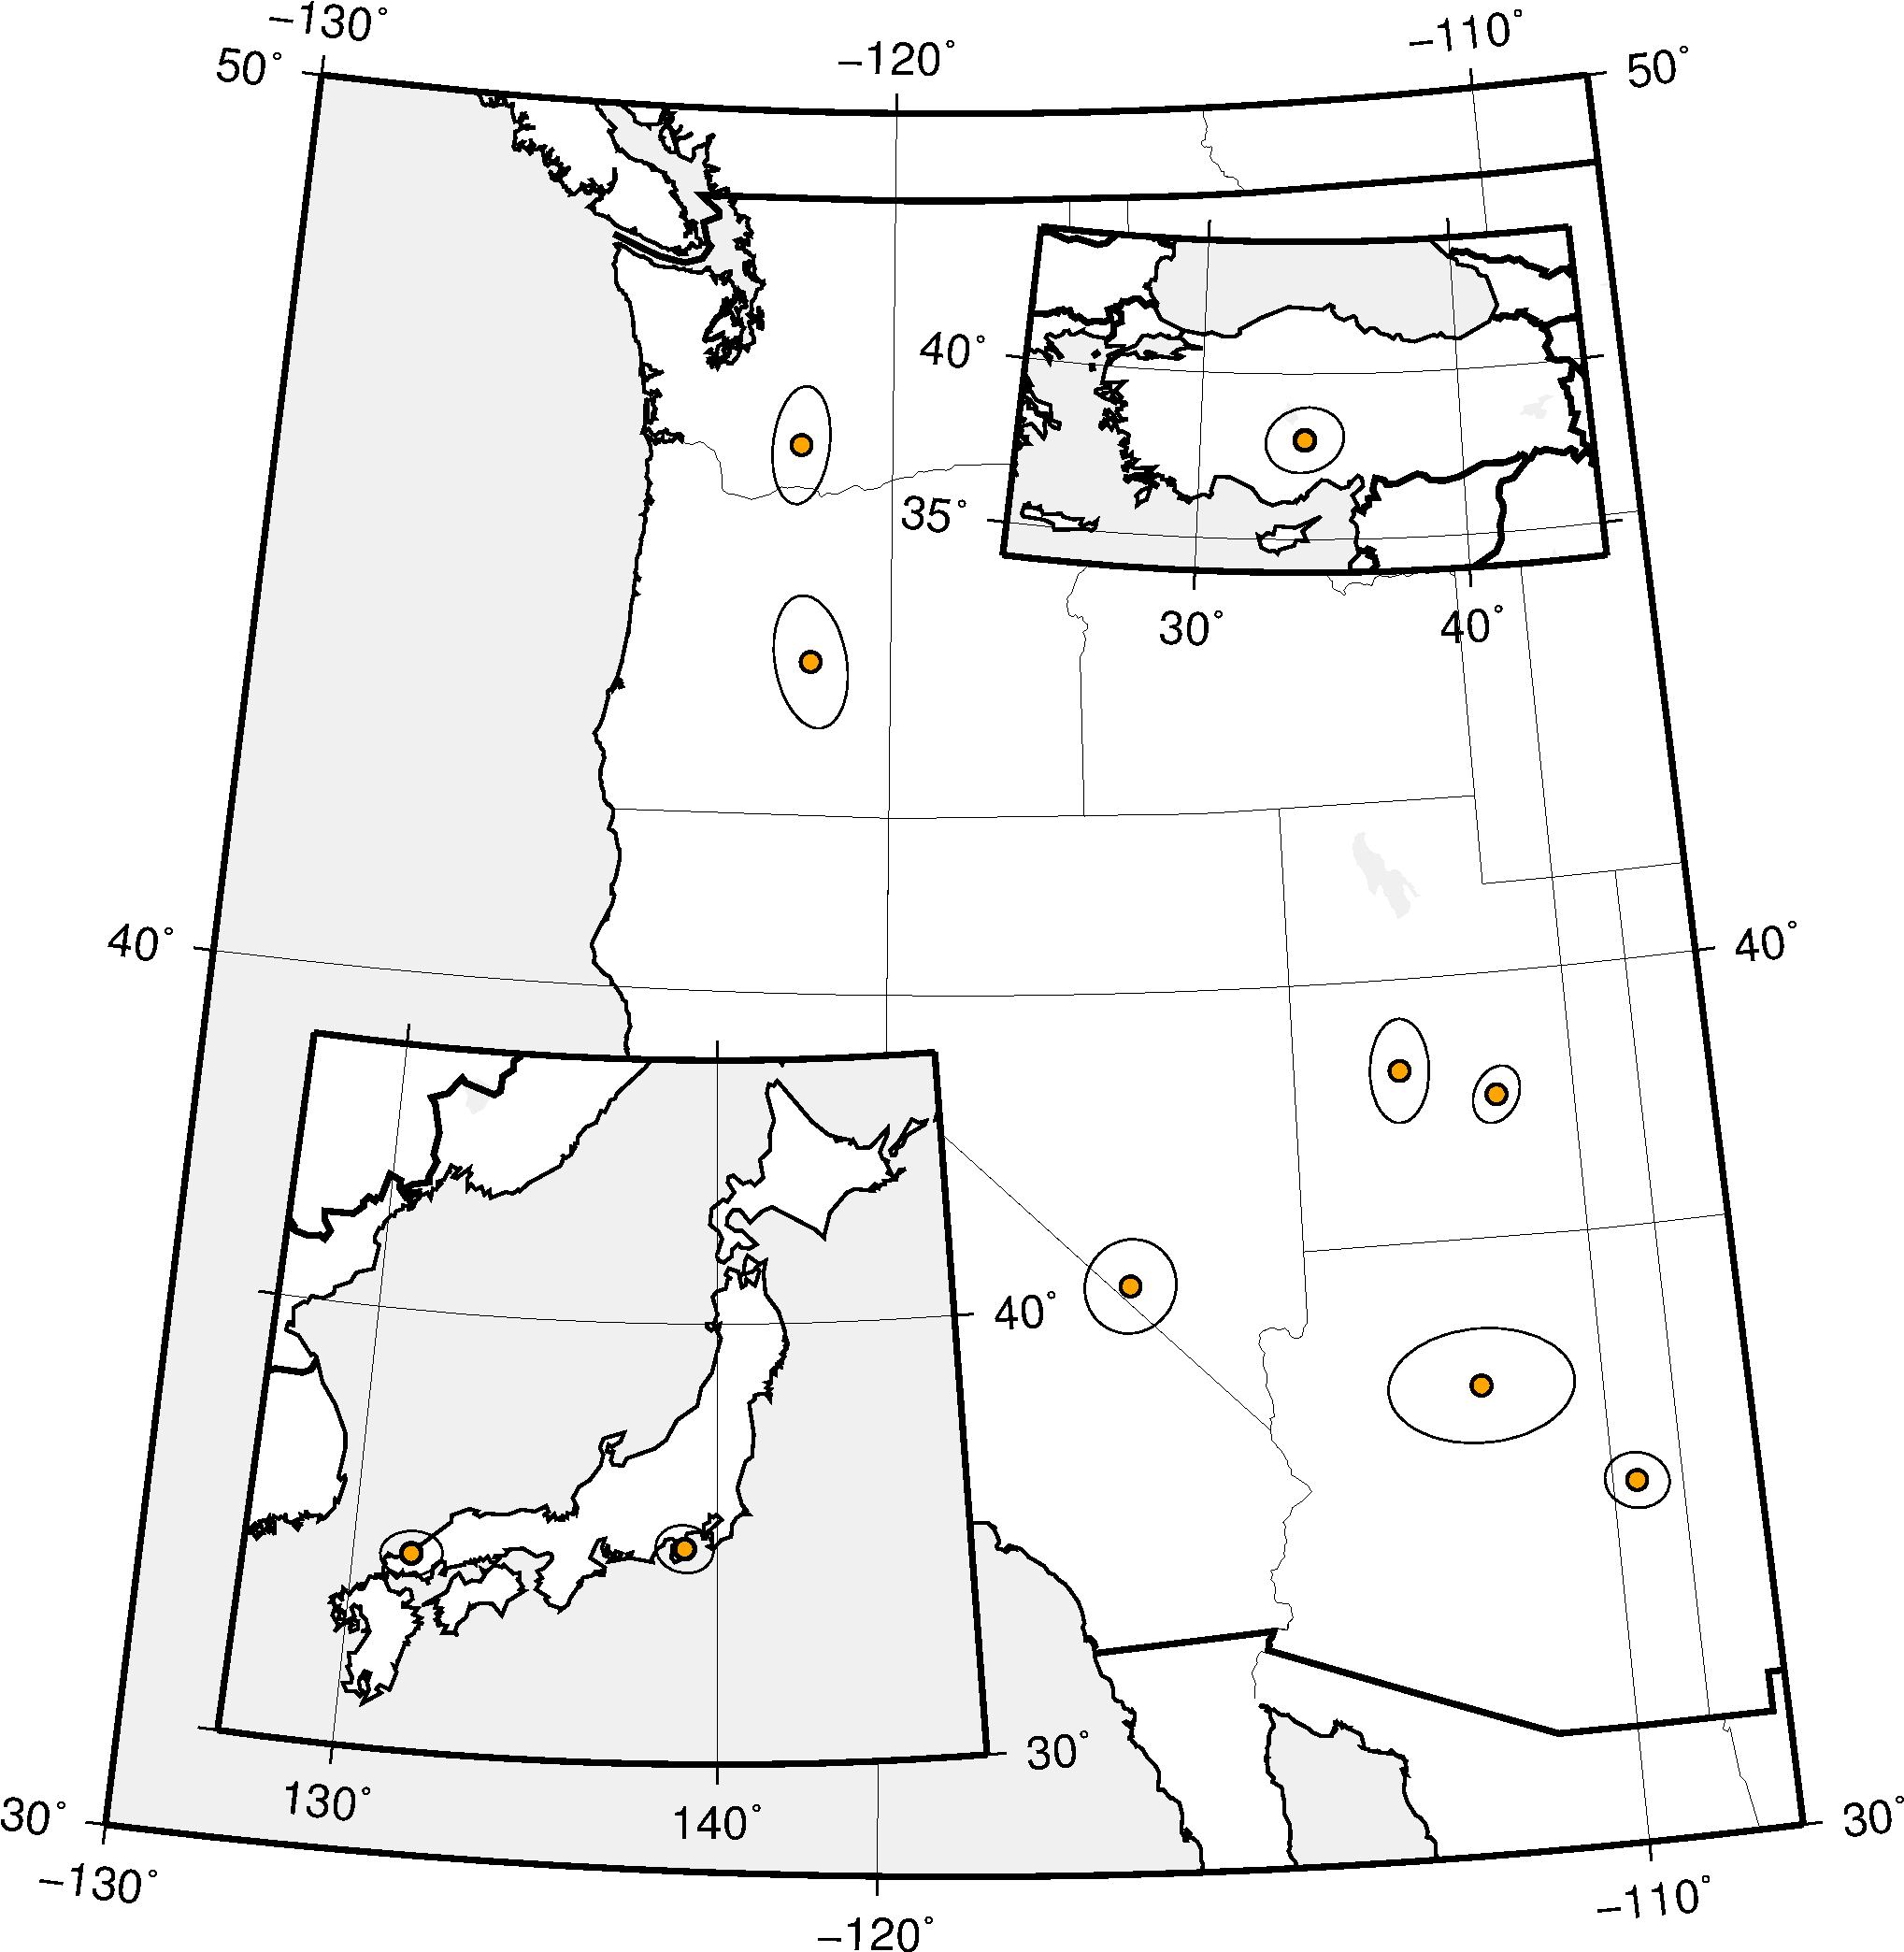
\includegraphics[width=0.5\linewidth]{figures/locators/earth_locator.png}
\caption{Locations of selected volcano clusters with their kernel bandwidth ellipses drawn over them. Ellipses are enlarged to show regional variation.}
\label{fig_earthlocator}
\end{figure}

\section{Discussion}
The major finding of this study is that the spatial density of vents between planets is generally different by an order of magnitude. On Earth, six monogenetic volcano clusters are shown to all cluster on the order of 0.1 vents per km$^2$. On Mars, two clusters have a vent density of around 0.001 vents per km$^2$. One cluster, in the basaltic caldera of Arsia Mons, is more focused by a factor of five. In between these vent densities, Venus shield fields have densities of 0.01 vent per km$^2$. Venus shield fields are still more focused than the regional shield plains, which have an average density of 0.003 vents per km$^2$, similar to the Arsia Mons cluster. Essentially, volcanic vents in Earth fields have 10s km$^2$ of space between neighboring vents, on Venus, distributed volcanoes have 100s km$^2$ of individual space, and on Mars, two of three fields have 1000s  km$^2$ of space between neighboring vents, while one is clustered on a ``Venusian'' scale.

\subsection{Geologic implications of the kernel bandwidth}
Each bandwidth ellipse mimicks attributes of its corresponding vent cluster and likely reflects geologic properties which effect the volcano cluster. The bandwidth ellipse area at one standard deviation (1-sigma) reflects both the spatial extent of volcanoes in the cluster and the number of vents in the cluster. Larger volcano clusters correlate with larger bandwidths ellipses, while clusters with more volcanoes in the same amount of space have smaller bandwidths. Because bandwidth area is perfectly correlated with these two characteristics, it is better to refer to each characteristic directly. Similarly, bandwidth ellipse elongation, or the difference in the major and minor axis standard deviations, is a function of the anisotropy in vent production through the cluster, either because of a farther extent of volcanoes in one direction or because of more vents per km in one direction. The anisotropy of vent production in a cluster can be explored using bandwidth elongation as a proxy.

Elongation of the bandwidth of a volcano cluster can be explained by one or a combination of at least three geologic processes. First, the magma source region underlying the volcano cluster might be elongated, matching the distribution of volcanoes observed at the planet's surface. Second, the magma source region might have migrated with time or multiple magma source regions that are spatially adjacent might be overprinting pre-existing populations. Third, the hydrodynamic conductivity of the crust might itself be anisotropic, preferrentially focusing magma in one direction or enabling magma to spread laterally away from a source region. While all three of these might apply to all volcanic fields in varying degrees of magnitude, I will discuss how the anisotropy seen in the bandwidth ellipse might be explained by one of these processes for example clusters.

\subsubsection{Elongated Source Region}
Cascadian volcanic fields are a good example of this.

\begin{figure}
\centering
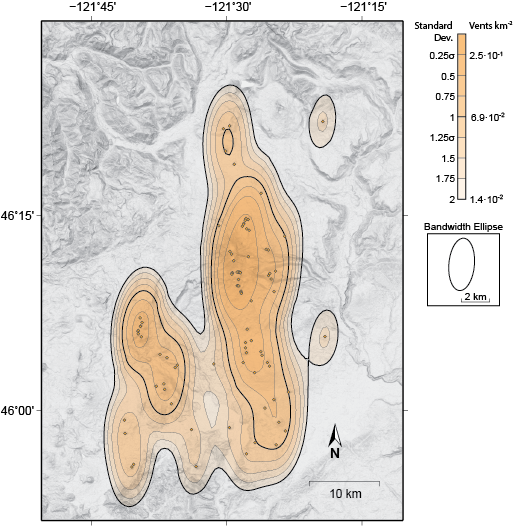
\includegraphics[width=0.6\linewidth]{figures/adams_kde_72dpi}
\caption{Volcanic vent density of monogenetic volcanoes near Mt. Adams (Washington, USA). If the magma source region is parallel to the subduction zone to the west, this might result in an elongated volcano distribution and kernel bandwidth ellipse.}
\label{fig_adamskde}
\end{figure}


\subsubsection{Magma source migration or multiple overprinting sources}
Springerville and San Francisco volcanic field are great examples of this, but Syria Planum might also be applicable.

\begin{figure}
\centering
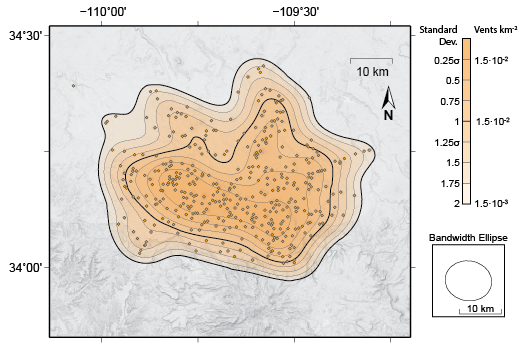
\includegraphics[width=0.6\linewidth]{figures/springerville_kde_72dpi}
\caption{Volcanic vent density of the Springerville Monogenetic Volcanic Field (Arizona, USA). The migration of the magma source with respect to the crust over time might be the source of the E-W elongated kernel ellipse.}
\label{fig_springervillekde}
\end{figure}


\subsubsection{Anisotropic crustal conductivity}
San Rafael and Arsia Mons are perfect for this example. Maybe the cascadian volcanoes as well but I'm not too sure.


\begin{figure}
\centering
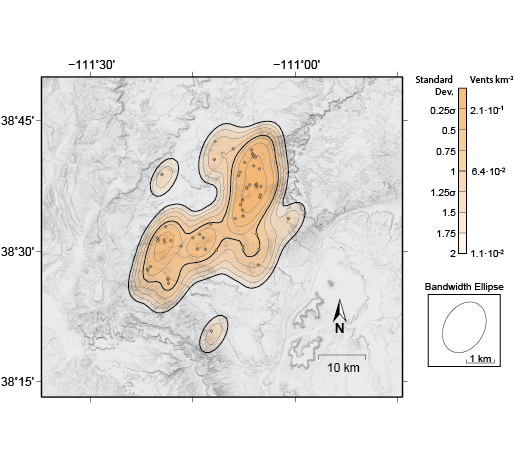
\includegraphics[width=0.6\linewidth]{figures/sanrafael_kde_72dpi}
\caption{Volcanic conduit density of the San Rafael Volcanic Field (Utah, USA). Dikes are oriented north following pre-existing joint sets in the upper crust, possibly influencing the shape of the kernel ellipse.}
\label{fig_sanrafaelkde}
\end{figure}


\subsection{Volume Flux Density}
Volume can also be compared with this method.
Spatial vent density and volume density compared across planets
We can compare km3/km2-a between the caribou field and arsia. We can compare km3/km2 between arsia and egrikuyu


\section{Conclusion}

\addcontentsline{toc}{section}{References}
\bibliographystyle{plainnat}
\bibliography{kde}

\section{Appendix: KDtools}
\label{sec_kdtoolscode}
Below are the functions as written in the kdtools python library. This library is available on github at \url{https://github.com/jarichardson/kdtools}.

\subsection{contourBySigma}
\begin{verbatim}
def contourBySigma(Z, 
  sigmas=[0.25,0.5,0.75,1.0,1.25,1.5,1.75,2.0,2.25,2.5,2.75,3.0],
  gridspacings=[1,1]):
  '''
  Identifies Density contour levels given Sigma thresholds.
  Contours define areas within which lay X% of the total field density
  e.g.: Within the Sigma-2.0 contour lies 95.4% of total field density.
        The density value of each contour decreases with increasing
        sigma.
  Requires a numpy array of density values (Z), with any shape.
  Optionally, provide a list of requested sigma thresholds, and the
  grid size as a 2 item list, to normalize the density.
  
  Outputs a dictionary of {sigma-level: density value}. If sigma-levels
  are not found (off the grid if the grid is too small), they will not
  be included in the dictionary.
  '''
  #find cumulative density that is used to pass the given
  #sigma thresholds in "contours"
  cum_thresholds = 2*(norm.cdf(sigmas)-norm.cdf(0))
  
  integrate = 0.0
  curcontour = 0
  densitycontours = {}
  
  #sort and reverse Z
  Z = numpy.sort(Z,kind='quicksort',axis=None)[::-1]
  
  #assuming density units are m^-2, but spacing is not 1 cell m^-2
  #reduce cumulative threshold by grid resolution
  cum_thresholds *= 1.0/(gridspacings[0]*gridspacings[1])
  
  for i,d in enumerate(Z):
    integrate+=d
    #if the elapsed density surpasses the next contour
    if (integrate >= cum_thresholds[curcontour]):
      densitycontours[sigmas[curcontour]] = d
      curcontour += 1
      if (curcontour>=len(sigmas)):
        break
  
  return densitycontours
\end{verbatim}

\subsection{densityToRaster}
\begin{verbatim}
def densityToRaster(griddata, ranges, spacings, outrastername, clon=-999, 
  utmzone=-999, planet='earth', driver='GTiff', outproj="tm"):
  '''
  Outputs a 2-D array to a gdal-readable raster. Input expected to be
  in a transverse mercator projection.
  griddata: 2D data array
  outrastername: file name of raster output. If meter output is desired,
     it would be good practice to define clon or utm zone
  planet: 'earth','venus', or 'mars'. This is only needed to translate to
     latlong projections
  clon: center longitude of non-earth transverse mercator data
  utmzone: utm zone of earth data
  driver: gdal-readable raster short name [GTiff]
  outproj: 'tm' or 'll' for transverse mercator (no tranformation occurs)
     or latlong (gdalwarp will be implemented). [tm]
     
  ISSUES: If values are very low (normal for density grids), gdalwarp 
       doesn't work, so it is suggested that output remain in meters.
       A workaround might be to supply log10 values of griddata.
  '''
  
  #print an extra line for good looks
  print ""
  
  #Check that the user's requested driver will actually work before
  #doing anything
  userdriver = gdal.GetDriverByName(driver)
  if userdriver==None:
    print '\nerror: Raster type "'+driver+'" not a valid gdal driver!'
    print '  No map created.'
    return None
  
  gdaldriver = gdal.GetDriverByName('GTiff')
  gdaldriver.Register()
  cols = numpy.shape(griddata)[1]
  rows = numpy.shape(griddata)[0]
  bands = 1
  
  griddata = griddata[::-1]
  
  dest_raster = gdaldriver.Create(outrastername, cols, rows, bands, \
    gdal.GDT_Float64 )

  #adfGeoTransform[0] /* top left x */
  #adfGeoTransform[1] /* w-e pixel resolution */
  #adfGeoTransform[2] /* rotation, 0 if image is "north up" */
  #adfGeoTransform[3] /* top left y */
  #adfGeoTransform[4] /* rotation, 0 if image is "north up" */
  #adfGeoTransform[5] /* n-s pixel resolution */  
  geotrans = [ranges[0][0],spacings[0],0,ranges[1][1],0,(-1*spacings[1])]
  dest_raster.SetGeoTransform(geotrans)
  
  #set transverse mercator projection
  if (utmzone>=1 and utmzone<=60):
    srs = osr.SpatialReference()
    srs.SetUTM( utmzone, 1 ) #1 means north, this could be problematic
    srs.SetWellKnownGeogCS( 'WGS84' );
    dest_raster.SetProjection( srs.ExportToWkt() )

  elif (clon>=-360 and clon<=360):
    srs = osr.SpatialReference()
    
    if (planet == 'venus'):
      srs.ImportFromProj4( '+proj=tmerc +lat_0=0 +lon_0='+str(clon)+ \
        ' +k=0.9996 +x_0=0 +y_0=0 +a=6051800 +b=6051800 +units=m +no_defs' )
      srs.SetProjCS( "Venus 2000 Sphere, Custom Meridian" )
      srs.SetGeogCS( 'Venus 2000', 'D_Venus_2000', 'Venus_2000_IAU_IAG', \
        6051800.0, 0.0 )
    
    elif (planet == 'mars'):
      srs.ImportFromProj4( '+proj=tmerc +lat_0=0 +lon_0='+str(clon)+ \
        ' +k=0.9996 +x_0=0 +y_0=0 +a=3396190 +b=3396190 +units=m +no_defs' )
      srs.SetProjCS( "Mars 2000 Sphere, Custom Meridian" )
      srs.SetGeogCS( 'Mars 2000', 'D_Mars_2000', 'Mars_2000_IAU_IAG', \
        3396190.0, 169.89444722361179 )
    else:
      print '\nwarning: clon set but planet is not venus or mars.'
      print '  output raster will not have projection metadata'
      #return 0
    dest_raster.SetProjection( srs.ExportToWkt() )
  
  dest_raster.GetRasterBand(1).WriteArray( griddata )
  dest_raster = None
  
  #warp to ll if necessary
  if outproj=='ll':
    if planet=='earth':
      #catch invalid utmzone
      if ((utmzone<1) or (utmzone>60)):
        print 'utm zone not valid (1-60). Cannot create latlong raster.'
        print 'utm raster saved at '+outrastername
        return 0
      
      #reproject the transverse mercator grid
      os.system('gdalwarp -r cubic -t_srs "+proj=longlat +datum=WGS84" '+ \
        outrastername+' tmpLL.tif')
      
    #if not earth, catch invalid center_lon
    elif ((clon<-360) or (clon>360)):
      print 'center longitude not valid (-360 to 360).', \
        ' Cannot create latlong raster.'
      print 'transverse mercator raster saved at '+outrastername
      return 0
    else:
      if planet=='mars':
        radius='3396190'
      elif planet=='venus':
        radius='6051800'
      else:
        print 'planet not either earth, venus, or mars.', \
          ' cannot create latlong raster.'
        print 'transverse mercator raster saved at '+outrastername
        return 0
      
      #reproject the transverse mercator grid
      os.system('gdalwarp -r cubic -t_srs "+proj=longlat +k=0.9996 '+ \
        '+x_0=0 +y_0=0 +a='+radius+' +b='+radius+' +no_defs" '+ \
        outrastername+' tmpLL.tif')
      
    #overwrite the transverse meter raster with the longlat raster file
    if driver=='GTiff':
      os.system('mv tmpLL.tif '+outrastername)
    else:
      os.system('gdal_translate -of '+driver+' tmpLL.tif '+outrastername)
      os.remove('tmpLL.tif')
  
  #If output is in meters, but user wants a non-Tiff, change format here
  elif driver!='GTiff':
    os.system('gdal_translate -of '+driver+' '+outrastername+' tmpM.tif')
    os.system('mv tmpM.tif '+outrastername)
  
  if os.path.isfile('tmpM.aux.xml'):
    os.remove('tmpM.aux.xml')
  if os.path.isfile('tmpLL.aux.xml'):
    os.remove('tmpLL.aux.xml')
  if os.path.isfile(outrastername+'.aux.xml'):
    os.remove(outrastername+'.aux.xml')
  
  return 0
\end{verbatim}

\subsection{ellipseGen}
\begin{verbatim}
def ellipseGen(bd,eps=False,epsfilename='bandwidth_ellipse.eps'):
  '''
  Identifies the major and minor axes directions and standard
  deviations of a Gaussian ellipse defined by a 2x2 covariance
  matrix. Precision is to the nearest degree.
  
  Prints out solution, and optionally uses GMT to draw the ellipse
  to epsfilename, if eps=True.
  
  Outputs major-axis direction, major-axis standard deviation, and
          minor-axis standard-deviation.
  '''
  detH = linalg.det(linalg.sqrtm(bd)) #determinate sqrt bandwidth
  invH = linalg.inv(linalg.sqrtm(bd)) #inverse sqrt bandwidth
  constant = 2.0*numpy.pi*detH
  
  radius = 20
  angles = numpy.arange(0,numpy.pi,(numpy.pi/180.0))
  D = numpy.zeros(len(angles))
  
  #simulate density in all directions
  for i,phi in enumerate(angles):
    dx = radius*numpy.cos(phi)
    dy = radius*numpy.sin(phi)
    dxdy = numpy.dot(invH,numpy.array([[dx],[dy]]))
    dist = numpy.dot(numpy.transpose(dxdy),dxdy)[0][0]
    D[i] = numpy.exp(-0.5*dist)/constant
  
  #Find azimuth of greatest, least density
  maxaz = angles[numpy.where(D==max(D))][0]
  minaz = angles[numpy.where(D==min(D))][0]
  
  #Calculate Density at vent location
  dxdy = numpy.dot(invH,numpy.array([[0],[0]]))
  dist = numpy.dot(numpy.transpose(dxdy),dxdy)[0][0]
  ventD = numpy.exp(-0.5*dist)/constant
  
  #Calculate standard deviations
  #For the major axis
  majsd = (10*(2**0.5))/(-1*numpy.log(max(D)/ventD))**0.5 #(radius=20 units)
  majdir = 90-numpy.degrees(maxaz) #Gives direction from North. East is +
  #For the minor axis
  minsd = (10*(2**0.5))/(-1*numpy.log(min(D)/ventD))**0.5
  mindir = 90-numpy.degrees(minaz)

  #Print out the results
  '''
  print '\nBandwidth Ellipse Information'
  print 'major axis:'
  print ('  degrees from north - %0.0f' % majdir)
  print ('  standard deviation - %0.4f' % majsd)
  print 'minor axis:'
  print ('  degrees from north - %0.0f' % mindir)
  print ('  standard deviation - %0.4f' % minsd)
  '''
  
  if eps==True:
    majaxis = 2*majsd
    minaxis = 2*minsd
    
    with open('ellipseGMT.xy','w') as f:
      f.write('0\t0\t%0.0f\t%0.4f\t%0.4f' % (majdir, majaxis, minaxis))
    os.system('psxy ellipseGMT.xy -SE -Wblack -JX6i ' + \ 
      ('-R%0.4f/%0.4f/%0.4f/%0.4f -Ba%0.4f -K >' % ((-1*majaxis),majaxis, \
      (-1*majaxis), majaxis, majsd)) + epsfilename)
    os.remove('ellipseGMT.xy')      
    print ('\nPlotted ellipse at '+epsfilename)
    
  returnstats = [majdir,majsd,minsd]
  return returnstats
\end{verbatim}

\subsection{KD}
\begin{verbatim}
def KD(bd,coors,ranges,spacings,weights=[]):
  '''
  Estimates point density using:
  bd       - a kernel bandwidth (2x2 covariance  matrix)
  coors    - 2xN list of coordinates for N points.
  ranges   - a 2x2 [[W,E],[S,N]] array
  spacings - a 1x2 [X-resolution,Y-resolution] array
  weights  - a 2xN list of wieghts for N points [None]
  
  Outputs X,Y,D: Eastings, Northings, and Densities in a Meshgrid
  format (i.e. X will be tiled, Y will be repeated)
  '''
  
  #If weights are given, test to see that they're valid
  if weights != []:
    if numpy.shape(weights)[0] != numpy.shape(coors)[0]:
      print "error: weight array not same length as coordinate array!"
      print "  cannot create kernel density map."
      return None
  #If weights are not given, make weights even across the board
  else:
    weights = numpy.ones(len(coors))
  
  weightaverage = numpy.sum(weights)/len(weights)
  
  detH = linalg.det(linalg.sqrtm(bd)) #determinate sqrt bandwidth
  invH = linalg.inv(linalg.sqrtm(bd)) #inverse sqrt bandwidth
  
  #constant variable in gaussian pdf
  constant = 2.0*numpy.pi*detH*len(coors) * weightaverage

  #define map grid
  x = numpy.arange(ranges[0][0],(ranges[0][1]+spacings[0]),spacings[0])
  y = numpy.arange(ranges[1][0],(ranges[1][1]+spacings[1]),spacings[1])
  X,Y = numpy.meshgrid(x,y)  #X and Y are now tiled to grid
  D = numpy.zeros(numpy.shape(X)) #Density Grid
  dist = numpy.zeros(numpy.shape(X)) #distance matrix grid
  
  #Three for loop with enumerates... Nick Voss would be proud.
  for w,v in enumerate(coors):
    for i,e in enumerate(x):
      for j,n in enumerate(y):
        dx = e-v[0]
        dy = n-v[1]
        dxdy = numpy.dot(invH,numpy.array([[dx],[dy]]))
        dist[j][i] = numpy.dot(numpy.transpose(dxdy),dxdy)[0][0]
    D += numpy.exp(-0.5 * dist) * weights[w]
  
  D /= constant #normalize
  
  return X,Y,D
\end{verbatim}

\subsection{main}
\begin{verbatim}
def main():
  '''
  runs tests for kdtools functions using a synthetic dataset
  some tests are visual and require matplotlib
  '''
  import matplotlib.pyplot as plt
  from matplotlib.ticker import LogFormatter 
  
  #create a random synthetic dataset of points
  data = numpy.random.uniform(31,35,[50,2])
  
  #or create a grid of synthetic points
  #data = numpy.zeros([100,2])
  #data_easts  = numpy.linspace(31,35,10)
  #data_norths = numpy.linspace(31,35,10)
  #E, N = numpy.meshgrid(data_easts,data_norths)
  #data[:,0] = E.reshape((100))
  #data[:,1] = N.reshape((100))
  
  data[:,1] *= 1.3 #stretch data in the N-S direction
  zone = 36   #utm zone on earth for this lat-long
  clon = 33.0 #center longitude of data on other planets
  
  #random synthetic weights
  weights = numpy.random.uniform(1,20,len(data))
  #weights = numpy.linspace(1,20,len(data)) #this puts the weights in order
  
  print "\nsynthetic dataset info"
  print "  %d points on an x,y grid" % len(data)
  print "  x min,mean,max - %0.3f, %0.3f, %0.3f" % (min(data[:,0]), \ 
    (sum(data[:,0])/len(data)),max(data[:,0]))
  print "  y min,mean,max - %0.3f, %0.3f, %0.3f" % (min(data[:,1]), \
    (sum(data[:,1])/len(data)),max(data[:,1]))
  
  #create grid matrix
  gridresolution = [10000,10000]
  
  
  #1. reproject(llcoors, planet='earth', utmzone=-999, clon=-999)
  data = reproject(data,planet='mars',clon=clon)
  print "\nReprojected synthetic dataset info"
  print "  %d points on an x,y grid" % len(data)
  print "  x min,mean,max - %0.3f, %0.3f, %0.3f" % (min(data[:,0]), \
    (sum(data[:,0])/len(data)),max(data[:,0]))
  print "  y min,mean,max - %0.3f, %0.3f, %0.3f" % (min(data[:,1]), \
    (sum(data[:,1])/len(data)),max(data[:,1]))
  
  #2. rangeBuffer(coords, B=0)
  datarange = rangeBuffer(data,B=30)
  print "\ndata range with 30% buffer:\n", datarange
  
  #3. samse_bandwidth(coords)
  bandwidth = samse_bandwidth(data)
  if len(bandwidth) == 0:
    print "samse_bandwidth returned an error"
    return None
  print "\nsamse bandwidth:\n", bandwidth
  

  #4. ellipseGen(bd, eps=False, epsfilename='bandwidth_ellipse.eps')
  ellipse_stats = ellipseGen(bandwidth, eps=True)
  print "\nellipse stats:"
  print "  ellipse major axis orientation (deg N) - ", ellipse_stats[0]
  print "  ellipse major axis standard deviation  - ", ellipse_stats[1]
  print "  ellipse minor axis standard deviation  - ", ellipse_stats[2]
  
  #5. KD(bd, coors, ranges, spacings)
  print "\nCalculating Density on grid..."
  (X,Y,D) = KD(bandwidth, data, datarange, gridresolution, weights=weights)
  
  integrateddensity = numpy.sum(D)*gridresolution[0]*gridresolution[1]
  print ("  Total Density within grid - %0.3f%%" % (integrateddensity*100))
  print ("  Maximum Density on grid   - %0.3e sq. unit area^-1" % \
    numpy.amax(D))
    
  
  #6. contourBySigma(Z, sigmas, gridspacings)
  contours = contourBySigma(D, sigmas=[0.5,1,2], \ 
    gridspacings=gridresolution)
  print "\nDensity value contours at"
  print "  0.5-sigma: %0.3e sq. unit area^-1" % contours[0.5]
  print "    1-sigma: %0.3e" % contours[1]
  print "    2-sigma: %0.3e" % contours[2]
  
  
  #7. densityToRaster(griddata, ranges, spacings, outrastername, clon=-999, 
  #              utmzone=-999, planet='earth', driver='GTiff', outproj='tm')
  gdalerr = densityToRaster(numpy.log10(D), datarange, gridresolution, \
    'synth.grd', clon=clon, planet='mars', outproj='ll', driver="GMT")
  if gdalerr != -1:
    print "\nOutput test raster to synth.tif"
  
  #8. Plot the results
  print "\nPlotting Density map with points"
  plt.clf()
  plt.subplot(1, 1, 1)
  plt.title('test density (points per square unit)')
  # set the limits of the plot to the limits of the data
  plt.axis([datarange[0][0], datarange[0][1], datarange[1][0], \
    datarange[1][1]])
  
  #Color plot of the density data from KD
  plt.pcolor(X, Y, D, cmap='YlOrRd', vmin=0, vmax=numpy.amax(D))
  #format the color bar labels to log scale
  formatter = LogFormatter(10, labelOnlyBase=False) 
  plt.colorbar(format=formatter)
  
  #Contour plot from contourBySigma
  contourlevels = [contours[0.5],contours[1],contours[2]]
  CS = plt.contour(X,Y,D,contourlevels,colors='k')
  plt.clabel(CS, fontsize=9, inline=1, fmt=formatter)
  
  #Scatter Plot of synthetic dataset
  plt.scatter(data[:,0],data[:,1],c='k',s=(weights**2),marker='.')
  plt.show()
\end{verbatim}

\subsection{rangeBuffer}
\begin{verbatim}
def rangeBuffer(coords,B=0):
  '''
  Creates a buffer of B% [default 0%, no buffer] around 
  N-dimensional data. Input should be a numpy array.
  Output will be 2xN array, with min, max of each dimension in
  columns 1 and 2, respectively.
  
  ex: 
  data         range output
  [[1,5],      [[0,2],
   [2,5],  =>   [4,9]]
   [0,4],
   [1,9]]
  '''
  extents = numpy.ones([numpy.shape(coords)[1],2])
  for dim in range(numpy.shape(coords)[1]):
    data = coords[:,dim]
    dataRange = data.max() - data.min()
    bufsize = dataRange*(B/100.0)
    extents[dim,0] = data.min() - bufsize
    extents[dim,1] = data.max() + bufsize
    
  return extents
\end{verbatim}

\subsection{reproject}
\begin{verbatim}
def reproject(llcoors,planet="earth",utmzone=-999,clon=-999,inverse=False):
  '''
  Reprojects long-lat data into transverse mercator coordinates
  with units of meters. Optionally, set inverse=True to change
  transverse mercator to long-lat.
  
  Input should be numpy 2-col long, lat array.
  Output will be numpy 2-col easting, northing array.  
  
  Planet options: 'earth', 'venus', or 'mars'
  Earth requires a valid UTM zone
  Venus and Mars require a valid center longitude of the dataset
  
  Earth Transverse Mercator fit to WGS84 datum
  Venus Transverse Mercator fit to Spheriod of radius 6051800 m
  Mars Transverse Mercator fit to Spheriod of radius 3396190 m
  '''
  
  if planet == "earth":
    if (utmzone<1) or (utmzone>60):
      print "error in reproject:", \
        " utm zone not set correctly (1<=utmzone<=60)"
      return 0
    TransMerc = pyproj.Proj('+proj=utm +datum=WGS84 +zone='+str(utmzone))
  elif planet == "venus":
    if (clon<-360) or (clon>360):
      print "error in reproject: ", \
        "center longitude not set correctly (-360<=clon<=360)"
      return 0
    TransMerc = pyproj.Proj('+proj=tmerc +lat_0=0 +lon_0='+str(clon)+ \ 
      ' +k=0.9996 +x_0=0 +y_0=0 +a=6051800 +b=6051800 +units=m +no_defs')
  elif planet == "mars":
    if (clon<-360) or (clon>360):
      print "error in reproject: ",
        "center longitude not set correctly (-360<=clon<=360)"
      return 0
    TransMerc = pyproj.Proj('+proj=tmerc +lat_0=0 +lon_0='+str(clon)+ \
      ' +k=0.9996 +x_0=0 +y_0=0 +a=3396190 +b=3396190 +units=m +no_defs')
  else:
    print "error in reproject: planet not earth, venus, or mars."
    return 0
  
  if inverse==True:
    reproj = TransMerc(llcoors[:,0],llcoors[:,1])
    mcoors = numpy.transpose(reproj)
  else:
    reproj = TransMerc(llcoors[:,0],llcoors[:,1])
    mcoors = numpy.transpose(reproj)
  
  return mcoors
\end{verbatim}

\subsection{samse\_bandwidth}
\begin{verbatim}
def samse_bandwidth(coords):
  '''
  Evaluates the SAMSE Kernel in R using a coordinate list (coords).
  Returns 2x2 bandwidth covariance matrix.
  Requires: R, KS library in R.
  '''
  
  bandwidthfile='tmpbdR.out'
  datafile     ='tmpcrs.out'
  #Writes the data to a file for R
  numpy.savetxt(datafile,coords)
  
  #Writes the batch file that R will use
  with open('samse_batch.r','w') as f:
    f.write('library(ks)\n')
    f.write('data<-read.table("'+datafile+'")\n')
    f.write('bd <- Hpi(x=data,nstage=2,pilot="samse",pre="sphere")\n')
    f.write('sink("'+bandwidthfile+'")\n')
    f.write('show(bd)\n')
    f.write('sink()')
  
  #command to run the batch file
  os.system('R CMD BATCH samse_batch.r')
  
  #check for output file doesn't exist, fail
  if not os.path.isfile(bandwidthfile):
    print "error: Output from R was not successful."
    print "    Is R and the KS library installed?"
    return []
  
  
  #Extract the bandwidth matrix from the bandwidth txt file
  bandwidth = numpy.loadtxt(bandwidthfile,skiprows=1,usecols=(1,2))
  
  #remove all these temporary files
  os.remove('samse_batch.r')
  os.remove('samse_batch.r.Rout')
  os.remove(bandwidthfile)
  os.remove(datafile)
  
  return bandwidth
\end{verbatim}

%\begin{figure}
%\centering
%\includegraphics[width=\linewidth]{map_diff}
%\label{fig:map_diff}
%\end{figure}


\end{document}
